%%%%%%%%%%%%%%%%%%%%%%%%%%%%%%%%%%%%%%%%%%%%%
%% Represent categorical logic graphically %%
%%%%%%%%%%%%%%%%%%%%%%%%%%%%%%%%%%%%%%%%%%%%%

%% Pdf rendering - uncomment for html 
%\def\pgfsysdriver{pgfsys-tex4ht.def}          

\usepackage{tikz}
\usepackage{xstring}

\tikzstyle{every node}=[font=\tiny] 

%%%%%%%%%%%%%%%%%%%%%%%%%%%%%%%%
%% Draw squares of Opposition %%
%%%%%%%%%%%%%%%%%%%%%%%%%%%%%%%%

\def\oppsquare{%
  \draw (-1.4,1) node[above left]{\textbf{A}} -- (1.4,1) node[above right]{\textbf{E}};%
  \draw (1.5,0.9) --(1.5,-0.9) node[below right]{\textbf{O}};%
  \draw (1.4,-1) -- (-1.4,-1) node[below left]{\textbf{I}};%
  \draw (-1.5,-0.9) -- (-1.5,0.9);%
}
\def\oppcross{%
  \draw (-1.3,0.8) -- (1.3,-0.8) node[sloped,above,pos=0.3]{contra} node[sloped,above,pos=0.7]{dictory};%
  \draw (-1.3,-0.8) -- (1.3,0.8) node[sloped,above,pos=0.3]{contra} node[sloped,above,pos=0.7]{dictory};%
}

\def\sqroppMod{%
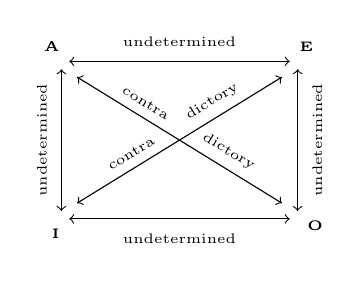
\begin{tikzpicture}
  \begin{scope}[<->]
    \oppsquare
    \oppcross
    \node[rotate=90] at (-1.75,0) {undetermined};
    \node at (0,1.25) {undetermined};
    \node at (0,-1.25) {undetermined};
    \node[rotate=90] at (1.75,0) {undetermined};
  \end{scope}
\end{tikzpicture}
}

\def\sqroppTrad{%
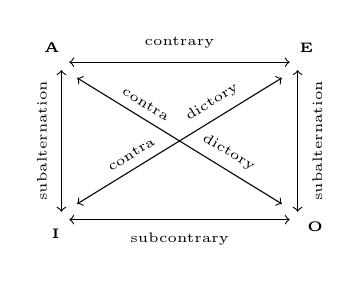
\begin{tikzpicture}
  \begin{scope}[<->]
    \oppsquare
    \oppcross
    \node[rotate=90] at (-1.75,0) {subalternation};
    \node at (0,1.25) {contrary};
    \node at (0,-1.25) {subcontrary};
    \node[rotate=90] at (1.75,0) {subalternation};
  \end{scope}
\end{tikzpicture}
}

%%%%%%%%%%%%%
%% Circles %%
%%%%%%%%%%%%%

%% Venn circles
\def\firstcircle{(0,0) circle (1cm)} 
\def\secondcircle{(0:1.5cm) circle (1cm)}
\def\thirdcircle{(60:1.5cm) circle (1cm)}

%% Overlapping and disjoint circles
\def\firstcircleN{(0,0) circle (.75cm) node [below left=.25in] {$A$}}
\def\secondcircleN{(0:2cm) circle (.75cm) node [below right=.25in] {$B$}}
\def\firstcircleA{(0,0) circle (1.25cm) node [above right] {$A$}}
\def\secondcircleA{(.125,0) circle (.75cm) node [below left=.25in] {$B$}}

%%%%%%%%%%%%%%%%%%%%%%%%%%%
%% Venn diagram template %%
%%%%%%%%%%%%%%%%%%%%%%%%%%%

\newenvironment{catprop}[2]%
  {\begin{tikzpicture}%
    \begin{scope}%
      \draw (-1.5,-1.5) rectangle (3,1.5);%
      \draw \firstcircle node [below left=.25in] {#1};%
      \draw \secondcircle node [below right=.25in] {#2};%
    \end{scope}}%
  {\end{tikzpicture}}

\newenvironment{catsyll}%
  {\begin{tikzpicture}%
    \begin{scope}%
      \draw (-1.5,-1.5) rectangle (3,2.75);%
      \draw \firstcircle node [below left=.25in] {S};%
      \draw \secondcircle node [below right=.25in] {P};%
      \draw \thirdcircle node [above right=.25in] {M};%
    \end{scope}}%
  {\end{tikzpicture}}


%%%%%%%%%%%%%%%%%%%%%%%%%%%%%%%%%%%%%%%%%%%%%%%%%%%%%%%%%%%%%%%%%%%%%%%%%%%%%%%%%%%%%%%%%
%%                                 Propositions                                        %%
%%%%%%%%%%%%%%%%%%%%%%%%%%%%%%%%%%%%%%%%%%%%%%%%%%%%%%%%%%%%%%%%%%%%%%%%%%%%%%%%%%%%%%%%%

%%%%%%%%%%%%%%%%%%%%
%% Universal Defs %%
%%%%%%%%%%%%%%%%%%%%

\def\fillleft{%
  \begin{scope}[even odd rule]
    \clip \secondcircle (-1,-1) rectangle (1,1);
    \fill \firstcircle;
  \end{scope}
}

\def\fillmiddle{%
  \begin{scope}
    \clip \firstcircle;
    \fill \secondcircle;
  \end{scope}
}

\def\fillright{%
  \begin{scope}[even odd rule]
    \clip \firstcircle (-1,-1) rectangle (2.5,1);
    \fill \secondcircle;
  \end{scope}
}

\def\fillbox{%
  \begin{scope}
    \fill (-1.5,-1.5) rectangle (3,1.5);
    \fill[fill opacity=1, white] \firstcircle \secondcircle;
    \draw[black] \firstcircle \secondcircle;
  \end{scope}
}

%%%%%%%%%%%%%%%%%%%%%%
%% Existential Defs %%
%%%%%%%%%%%%%%%%%%%%%%

\def\xleft{%
  \node {x};
}
\def\xleftA{%
\draw (0,0) node [draw,rounded corners] {x};
}%

\def\xmiddle{%
  \node [right=.6cm] {x};
}
\def\xmidA{%
  \draw (.75cm,0) node [draw,rounded corners] {x};
}%

\def\xright{%
  \node [right=1.5cm] {x};
}

\def\xbox{%
 \node [below right=1.1cm] {x};
}

%%%%%%%%%%%%%%%%%%%%%% Proposition Fxn %%%%%%%%%%%%%%%%%%%%%
%%            Draw any categorical proposition            %%
%%       \propdiagram{Quality: +/- }{Quantity: U/E}       %%
%%  {Subject: [non-]<string>}{Predicate: [non-]<string>}  %%
%%%%%%%%%%%%%%%%%%%%%%%%%%%%%%%%%%%%%%%%%%%%%%%%%%%%%%%%%%%%

\newcommand{\propdiagram}[5][blue]{%
\begin{scope}[fill opacity=0.5,#1]
  \IfStrEq{#4}{#5}{\PackageError{propdiagram}{Undefined option to tree: same term}{}}{}%
  \IfEqCase{#2}{%
    {+}{%
      \IfEqCase{#3}{%
        {U}{%
          \IfBeginWith{#4}{non}{%
            \IfBeginWith{#5}{non}{\fillright;}{\fillbox;}%
          }{%
            \IfBeginWith{#5}{non}{\fillmiddle;}{\fillleft;}%
          }%
        }%
        {E}{%
          \IfBeginWith{#4}{non}{%
            \IfBeginWith{#5}{non}{\xbox;}{\xright;}%
          }{%
            \IfBeginWith{#5}{non}{\xleft;}{\xmiddle;}%
          }%
        }%
      }%
    }%
    {-}{%
      \IfEqCase{#3}{%
        {U}{%
          \IfBeginWith{#4}{non}{%
            \IfBeginWith{#5}{non}{\fillbox;}{\fillright;}%
          }{%
            \IfBeginWith{#5}{non}{\fillleft;}{\fillmiddle;}%
          }%
        }%
        {E}{%
          \IfBeginWith{#4}{non}{%
            \IfBeginWith{#5}{non}{\xright;}{\xbox;}%
          }{%
            \IfBeginWith{#5}{non}{\xmiddle;}{\xleft;}%
          }%
        }%
      }%
    }%
  }%
\end{scope}

\def\proptitle{%
\begin{scope}[shift={(1.5cm,1.25cm)}]
  \IfEqCase{#2}{%
    {+}{%
      \IfEqCase{#3}{%
        {U}{\node {All #4 are #5};}%
        {E}{\node {Some #4 are #5};}%
      }%
    }%
    {-}{%
      \IfEqCase{#3}{%
        {U}{\node {No #4 are #5};}%
        {E}{\node {Some #4 are not #5};}%
      }%
    }%
  }[\PackageError{proptitle}{Title command must follow diagram command}{}]%%
\end{scope}
}
}


%%%%%%%%%%%%%%%%%%%%%%%%%%%%%%%%%%%%%%%%%%%%%%%%%%%%%%%%%%%%%%%%%%%%%%%%%%%%%%%%%%%%%%%%%
%%                                   Syllogisms                                        %%
%%%%%%%%%%%%%%%%%%%%%%%%%%%%%%%%%%%%%%%%%%%%%%%%%%%%%%%%%%%%%%%%%%%%%%%%%%%%%%%%%%%%%%%%%

%%%%%%%%%%%%%%%%%%%%%%%%%%% Existential Fxn 1 %%%%%%%%%%%%%%%%%%%%%%%%%%%%%%%%
%%      Place an X in any region (choice of color and whether circled)      %%
%%    Any combination of S,P,M represents intersection of those circles     %%
%%         \syllx[color]{Commitment: y/n}{region: combo of SPM}             %%
%%%%%%%%%%%%%%%%%%%%%%%%%%%%%%%%%%%%%%%%%%%%%%%%%%%%%%%%%%%%%%%%%%%%%%%%%%%%%%

\newcommand{\syllx}[3][black]{%
  \begin{scope}[#1]
  \IfStrEq{#2}{y}{\tikzstyle{every node}=[font=\tiny, draw, rounded corners]}{}%
  \StrLen{#3}[\region]%
  \IfEq{\region}{3}{\draw (30:0.85cm) node {X};}{}%
  \IfEqCase{#3}{%
    {SP}{\draw (0:0.75cm) node {X};}%
    {PS}{\draw (0:0.75cm) node {X};}%
    {SM}{\draw (60:0.75cm) node {X};}%
    {MS}{\draw (60:0.75cm) node {X};}%
    {PM}{\draw (30:1.4cm) node {X};}%
    {MP}{\draw (30:1.4cm) node {X};}%
  }%
  \IfEqCase{#3}{%
    {S}{\draw (0:0cm) node {X};}%
    {P}{\draw (0:1.5cm) node {X};}%
    {M}{\draw (60:1.5cm) node {X};}%
  }%
  \end{scope}
}% 

%%%%%%%%%%%%%%%%%%%%%%%%%%%%%%% Existential Fxn 2 %%%%%%%%%%%%%%%%%%%%%%%%%%%%%%%%%%%%%%%%%%
%%   Place an X on line between any two regions (choice of color and whether circled)     %%
%%      Function represents the existential proposition corresponding to the line         %%
%%          \syllxline[color]{Quality: +/-}{Subject: S/P/M}{Predicate: S/P/M}             %%
%%%%%%%%%%%%%%%%%%%%%%%%%%%%%%%%%%%%%%%%%%%%%%%%%%%%%%%%%%%%%%%%%%%%%%%%%%%%%%%%%%%%%%%%%%%%

\newcommand{\syllxline}[4][black]{%
  \begin{scope}[#1]
  \IfStrEq{#3}{#4}{\PackageError{syllx2}{Undefined option to tree: same term}{}}{}%
  \IfStrEqCase{#2}{%
    {+}{%
      \IfStrEq{#3#4}{SM}{\draw (40:0.8cm) node {X};}{}%
      \IfStrEq{#3#4}{SP}{\draw (20:0.8cm) node {X};}{}%
      \IfStrEq{#3#4}{MP}{\draw (30:1cm) node {X};}{}%
      \IfStrEq{#3#4}{MS}{\draw (40:0.8cm) node {X};}{}%
      \IfStrEq{#3#4}{PM}{\draw (30:1cm) node {X};}{}%
      \IfStrEq{#3#4}{PS}{\draw (20:0.8cm) node {X};}{}%
    }%
    {-}{%
      \IfStrEq{#3#4}{SM}{\draw (-20:0.55cm) node {X};}{}%
      \IfStrEq{#3#4}{SP}{\draw (75:0.55cm) node {X};}{}%
      \IfStrEq{#3#4}{MP}{\draw (70:1cm) node {X};}{}%
      \IfStrEq{#3#4}{MS}{\draw (40:1.5cm) node {X};}{}%
      \IfStrEq{#3#4}{PM}{\draw (-15:1cm) node {X};}{}%
      \IfStrEq{#3#4}{PS}{\draw (20:1.5cm) node {X};}{}%
    }%
  }[\PackageError{syllx2}{Undefined option to tree: quant}{}]%
  \end{scope}
}%


%%%%%%%%%%%%%%%%%%%%%%%%%%%%%%%% Universal Fxn %%%%%%%%%%%%%%%%%%%%%%%%%%%%%%%%%%
%%                Fill any region within the three circles                     %%
%%  Function represents the universal proposition corresponding to the region  %%
%%     \sylluniv[color]{Quality: All/No}{Subject: S/P/M}{Predicate: S/P/M}     %%
%%%%%%%%%%%%%%%%%%%%%%%%%%%%%%%%%%%%%%%%%%%%%%%%%%%%%%%%%%%%%%%%%%%%%%%%%%%%%%%%%

\newcommand{\sylluniv}[4][blue]{%
  \begin{scope}[fill opacity=0.5,#1]
    \IfStrEq{#3}{#4}{\PackageError{syllx2}{Undefined option to tree: same term}{}}{}%
    \IfStrEqCase{#2}{%
    {No}{%
      \IfSubStr{#3#4}{S}{%
        \IfSubStr{#3#4}{M}{%  
            \clip \firstcircle;
            \fill \thirdcircle;
        }{}%
        \IfSubStr{#3#4}{P}{%
            \clip \firstcircle;
            \fill \secondcircle;
        }{}%
      }{}%
      \IfSubStr{#3#4}{M}{%
        \IfSubStr{#3#4}{P}{%
            \clip \thirdcircle;
            \fill \secondcircle;
        }{}%
      }{}%
    }%
    {All}{%
      \IfStrEq{#3#4}{SM}{
          \clip \thirdcircle (-1.5,-1.5) rectangle (3,2.75);
          \fill[even odd rule] \firstcircle;
      }{}%
      \IfStrEq{#3#4}{SP}{
          \clip \secondcircle (-1.5,-1.5) rectangle (3,2.75);
          \fill[even odd rule] \firstcircle;
      }{}%
      \IfStrEq{#3#4}{MP}{
          \clip \secondcircle (-1.5,-1.5) rectangle (3,2.75);
          \fill[even odd rule] \thirdcircle;
      }{}%
      \IfStrEq{#3#4}{MS}{
          \clip \firstcircle (-1.5,-1.5) rectangle (3,2.75);
          \fill[even odd rule] \thirdcircle;
      }{}%
      \IfStrEq{#3#4}{PM}{
          \clip \thirdcircle (-1.5,-1.5) rectangle (3,2.75);
          \fill[even odd rule] \secondcircle;
      }{}%
      \IfStrEq{#3#4}{PS}{
          \clip \firstcircle (-1.5,-1.5) rectangle (3,2.75);
          \fill[even odd rule] \secondcircle;
      }{}%
    }%
  }[\PackageError{sylluniv}{Undefined option to tree: quant}{}]%
  \end{scope}
}

%%%%%%%%%%%%%%%%%%%%%% Commitment Fxn %%%%%%%%%%%%%%%%%%%%%%%%%%%%
%%  Add an X representing existential commitment to a syllogism %%
%%   \ecommit{Quality: +/-}{Subject: S/P/M}{Predicate: S/P/M}   %%
%%%%%%%%%%%%%%%%%%%%%%%%%%%%%%%%%%%%%%%%%%%%%%%%%%%%%%%%%%%%%%%%%%

\newcommand{\ecommit}[3]{%
  \begin{scope}
  \ifEq{#2}{#3}{\PackageError{ecommit}{Undefined option to tree: same term}{}}{
  \IfEqCase{#1}{%
    {+}{%
      \IfSubStr{#2#3}{M}{%
	\IfSubStr{#2#3}{S}{\draw (x:ycm) node [draw, rounded corners] {X};}{%
	  \ifSubStr{#2#3}{P}{\draw (x:ycm) node [draw, rounded corners] {X};}{}
	}
      }
      \IfStrEq{#2#3}{SP}{%
	{\draw (x:ycm) node [draw, rounded corners] {X};}
      }
    }
    {-}{%
      \IfSubStrBefore{#2#3}{M}{S}{\draw (x:ycm) node [draw, rounded corners] {X};}{}
      \IfSubStrBefore{#2#3}{M}{P}{\draw (x:ycm) node [draw, rounded corners] {X};}{}
      \IfSubStrBefore{#2#3}{S}{M}{\draw (x:ycm) node [draw, rounded corners] {X};}{}
      \IfSubStrBefore{#2#3}{P}{M}{\draw (x:ycm) node [draw, rounded corners] {X};}{}
      \IfSubStrBefore{#2#3}{S}{P}{\draw (x:ycm) node [draw, rounded corners] {X};}{}
    }
  }[\PackageError{ecommit}{Undefined option to tree: quant}{}]%
  }
  \end{scope}
}


